\documentclass[12pt, titlepage]{article}

\usepackage{fullpage}
\usepackage[round]{natbib}
\usepackage{multirow}
\usepackage{booktabs}
\usepackage{tabularx}
\usepackage{graphicx}
\usepackage{float}
\usepackage{hyperref}
\hypersetup{
    colorlinks,
    citecolor=black,
    filecolor=black,
    linkcolor=red,
    urlcolor=blue
}
\usepackage[round]{natbib}

\newcounter{acnum}
\newcommand{\actheacnum}{AC\theacnum}
\newcommand{\acref}[1]{AC\ref{#1}}

\newcounter{ucnum}
\newcommand{\uctheucnum}{UC\theucnum}
\newcommand{\uref}[1]{UC\ref{#1}}

\newcounter{mnum}
\newcommand{\mthemnum}{M\themnum}
\newcommand{\mref}[1]{M\ref{#1}}

\title{SE 3XA3: Design Documentation\\Minesweeper}

\author{Team 3, Banana Boat
		\\ Guiye Wu, 400089784
		\\ Shuying Chen, 400080161
		\\ Ace Huang, 400051063}

\date{\today}


\begin{document}

\maketitle

\pagenumbering{roman}
\tableofcontents
\listoftables
\listoffigures

\newpage
\begin{table}[h!]
\caption{\bf Revision History}
\begin{tabularx}{\textwidth}{p{3cm}p{2cm}X}
\toprule {\bf Date} & {\bf Version} & {\bf Notes}\\
\midrule
08/11/2018& 0.3 & Revision 0 complete\\
08/11/2018& 0.2 & Refined section\\
07/11/2018 & 0.1 & Draft of Sections\\
\bottomrule
\end{tabularx}
\end{table}

\newpage

\pagenumbering{arabic}

\section{Introduction}
\subsection{Overview}
This project is to redevelop a classic game minesweeper. The earliest minesweepers trace back to the 1960s, and this puzzle game style becomes popular during the 1980s. In modern time, minesweeper is the built-in game in window 7 system or the earlier version, for any other system it has to be downloaded in order to play this game. The game is very popular in earlier years, however, when the new systems are developed, the game is removed from the built-in games list and many people even don't know about the game nowadays. Our motivation is to renew this project and make it be well known. 
\subsection{Context}
This Module Guide(MG) is created after the Software Requirements Specification(SRS). The Module Guide specifies the modular structure of the system and is intended to allow both both designers and maintainers to easily identify the parts of the software. The SRS details all the functional and non-functional requirements for the project. The MG also shows how the software satisfies the functional and non-functional requirements as described in the SRS.
\\\\
When the MG is created, the Module Interaface Specification(MIS) will be created. The MIS will explain the semantics(state and environment variables, assumptions and access routines) and syntax of exported functions(input, output and exceptions) for each module, essentially providing further detail on each module that was specified in the MG.
% Citation: A. Bokhari, “Template Project,” 2017. [Online]. Available: https://gitlab.cas.mcmaster.ca/bokhari/se3xa3/blob/master/BlankProjectTemplate/Doc/Design/MG/MG.pdf. [Accessed: 08-Nov-2018].
%Citation: M. Calce, J. O. Fenster, and J. Tatasciore, “Module Guide,” Screen Holder Project, 2015. [Online]. Available: https://gitlab.cas.mcmaster.ca/screenholders/screenholders/blob/master/Documents/Rev1/ModuleGuide/ModuleGuide.pdf. [Accessed: 08-Nov-2018].
\subsection{Design Principles}
Information hiding and encapsulation are being used to guide the decomposition of the system into modules in the design principles, as well as the principle that a used relation should contain no cycles, have low coupling and high cohesion.\\\\
The principle of information hiding is that each module hides a secret from the rest of the system. The principle of encapsulation is that the changeable information is in the implementation of the module, but the module interface should not change when the implementation changes. Cycles in the uses relation means that module A uses module B which uses module A. This is considered poor design because it can cause infinite loops. Low coupling means that the modules are independent and do not use many other modules. High cohesion means that the elements within a module are strongly related.
% Citation: A. Bokhari, “Template Project,” 2017. [Online]. Available: https://gitlab.cas.mcmaster.ca/bokhari/se3xa3/blob/master/BlankProjectTemplate/Doc/Design/MG/MG.pdf. [Accessed: 08-Nov-2018].
%Citation: M. Calce, J. O. Fenster, and J. Tatasciore, “Module Guide,” Screen Holder Project, 2015. [Online]. Available: https://gitlab.cas.mcmaster.ca/screenholders/screenholders/blob/master/Documents/Rev1/ModuleGuide/ModuleGuide.pdf. [Accessed: 08-Nov-2018].
\subsection{Document Structure}
The documentation is organized as below:
\begin{itemize}
    \item Revision History for this document is listed before the introduction section.
    \item Section 2 lists the Anticipated and Unlikely Changes for this project's implementation. This will be used for traceability matrix in the following section.
    \item Section 3 gives the details about Module Hierarchy, by listing all the modules and their hierarchy.
    \item Section 4 explains the Connection Between Requirements and Design, which details the connection between the Modules and Software Requirements by their secret.
    \item Section 5 provide the Module Decomposition, which details the module name, secrets, and services for each module.
    \item Section 6 provides the Traceability Matrix. The first matrix connect the requirements with the modules, and the second one connects the anticipated changes with the modules.
    \item Section 7 provides Use Hierarchy Between Modules, which shows the use relations between modules.
\end{itemize}
\section{Anticipated and Unlikely Changes} \label{SecChange}
\subsection{Anticipated Changes}
AC1: The format of the input(mouse clicks).\\
AC2: The format of the output(image changes).\\
AC3: How the gaming frame changes from the level selection\\
AC4: How the game ending animation changes from the output of the game result.\\
AC5: How the timing changes from the input.\\
AC6: How the background music changes from the input.\\
AC7: Default settings for inputs.\\
\subsection{Unlikely Changes}
UC1: Input/output devices to the system(system assumes mouse and monitor are available.)\\
UC2: The animations of the winning/lose game.\\
UC3: The image of each particular type.\\
UC4: The level fram setting for each particular cetting.\\
UC5: The position of each cell and other functional frames.\\
UC6: The default settings.\\

\newpage
\section{Module Hierarchy} \label{SecMH}


\begin{table}[!htbp]
        \begin{tabular}{ll}
        \toprule
        Level 1 & Level 2 \\
        \midrule
        Hardware Hiding Module & \\
         \midrule
        Behaviour Hiding Module & Minesweeper Module \\
        & Board Module\\
        &Animation Module\\
        &Timer Module\\
		 \midrule
        Software Decision Module & Cell Module\\
        \bottomrule
        \end{tabular}
        \caption{Module Hierarchy}
        \label{Table 1}
        \end{table}
        
\begin{table}[!htbp]
	\begin{tabular}{ll}
		\toprule
		Module Name & Module Number \\
		\midrule
		Hardware Hiding Module & M1\\
		\midrule
		Minesweeper Module & M2\\
		\midrule
		Board Module & M3\\
		\midrule
		Animation Module & M4\\
		\midrule
		Timer Module & M5\\
		\midrule
		Cell Module & M6\\
		\bottomrule
	\end{tabular}
	\caption{Module Number Format}
	\label{Table 1}
\end{table}



\section{Connection Between Requirements and Design} \label{SecConnection}
The design of the system is intended to satisfy the requirements developed in the SRS(Software Requirement Specification). In this stage, the system is decomposed into modules. The connection between requirements and modules is listed in Table \ref{TblRT}. The Minesweeper Module initiates all the mouse action and connects all components together and ensures the program can be executed. The Cell Module creates the input cells and fill them up to the gaming frame. Appearance and usability requirements are satisfied through the Board Module as it deals with what elements are visible to the user and how they will interact with the program. The board module creates a user window that has all of the functions and capability available to user. \\
In order to make our designed easy and intuitive, the game was designed to use buttons for the selections. The buttons are clearly recognizable as to make it easier for the user to understand and make selection. The buttons are used to eliminate the chance of invalid input. The game is easy to install because it will be in an exe file. This means that the game will simply run if they have python and pygame installed on the system. Implementing this project in python also satisfies the requirement that the project should be able to run on different operations systems. In order to satisfy the requirement that the interface should be in position and clearly displayed, the various frame size will popped up based on the user's selection on the button. This ensures that the cells will always be in position. In order to satisfy players needs, the game is being kept simple and rebuilt as its original version as much as possible. This ensure that the flavour and the culture of the game are kept.
\section{Module Decomposition} \label{SecMD}
The following modules are decomposed to David Parnas' principle of information hiding. They are broken down in the following matter, \emph{Secret}, \emph{Service} and \emph{Implemented by}. Secret will describe in a single world what it is that the module is hiding. Services will detail what it is the module does and Implemented By states by what means the module is implemented.
\subsection{Hardware Hiding Modules (\mref{mHH})}
\begin{description}
\item[Secrets:] The implementation of virtual machine
\item[Services:] This module serves as the interface between software and hardware. This allows the system to communicate with the software the actions of all I/O.
\item[Implemented By:] Pygame and operating System
\end{description}

\subsection{Behaviour-Hiding Module}
\begin{description}
\item[Secrets:]Behaviours
\item[Services:] This module describes the visible behaviour of the application. It acts as the interpreter between
the Hardware Hiding Module and the Software Decision Module. This module ensures the software behavea as described in SRS(Software Requirement Specification).
\item[Implemented By:] N/A
\end{description}

\subsubsection{Minesweeper Module}
\begin{description}
\item[Secrets:] Initialization of mouse click action as input.
\item[Services:] Set the sizes of the frame and initialize the basic functionality and interface.
\item[Implemented By:] Pygame
\end{description}

\subsubsection{Board Module}
\begin{description}
\item[Secrets:] Dimension and the algorithm for setting up the frame
\item[Services:] Define and set the cell/frame and cells arrangements
\item[Implemented By:] Pygame
\end{description}

\subsubsection{Animation Module}
\begin{description}
\item[Secrets:]Algorithm for the winning/ lose animation
\item[Services:] Display different animation for win/lose situation.
\item[Implemented By:] Pygame
\end{description}

\subsubsection{Timer Module}
\begin{description}
\item[Secrets:] Algorithm for timing 
\item[Services:] Provide a timer to keep track of the user's playtime
\item[Implemented By:] Pygame
\end{description}

\subsection{Software Decision Module}

\subsubsection{Cell Module}
\begin{description}
\item[Secrets:]Algorithm for initialize the cells
\item[Services:] Initialize the cells with pictures
\item[Implemented By:] Pygame
\end{description}

\newpage
\section{Traceability Matrix} \label{SecTM}

This section shows two traceability matrices: between the modules and the
requirements and between the modules and the anticipated changes.

% the table should use mref, the requirements should be named, use something
% like fref
\begin{table}[H]
\centering
\begin{tabular}{p{0.2\textwidth} p{0.6\textwidth}}
\toprule
\textbf{Req.} & \textbf{Modules}\\
\midrule
\multicolumn{2}{c}{Functional Requirements}\\
\midrule
FR1 & M2,M3\\
FR2 & M2,M3\\
FR3 & M2,M3\\
FR4 & M2,M3\\
FR5 & M2,M3\\
FR6 & M2,M3,M4\\
FR7 & M2,M3\\
FR8 & M2\\
FR9 & M2,M3\\
FR10 & M2\\
FR11 & M2,M4\\
FR12 & M2,M4\\
FR13 & M2,M3\\
FR14 & M2,M3\\
FR15 & M2,M3\\
\midrule
\multicolumn{2}{c}{Non-functional Requirements}\\
\midrule
NFR1 & M3,M6\\
NFR2 & M2\\
NFR3 & M2\\
NFR4 & M6\\
NFR5 & M6\\
NFR6 & M3\\
NFR7 & M2,M3\\
NFR8 & M2,M3\\
NFR9 & M2\\
NFR10 & M1\\

\bottomrule
\end{tabular}
\caption{Trace Between Requirements and Modules}
\label{TblRT}
\end{table}

\begin{table}[H]
\centering
\begin{tabular}{p{0.2\textwidth} p{0.6\textwidth}}
\toprule
\textbf{AC} & \textbf{Modules}\\
\midrule
AC1 & M3\\
AC2 & M3\\
AC3 & M3\\
AC4 & M4\\
AC5 & M5\\
AC6 & M3\\
AC7 & M2\\
\bottomrule
\end{tabular}
\caption{Trace Between Anticipated Changes and Modules}
\label{TblACT}
\end{table}

\section{Use Hierarchy Between Modules} \label{SecUse}


\begin{figure}[H]
\centering
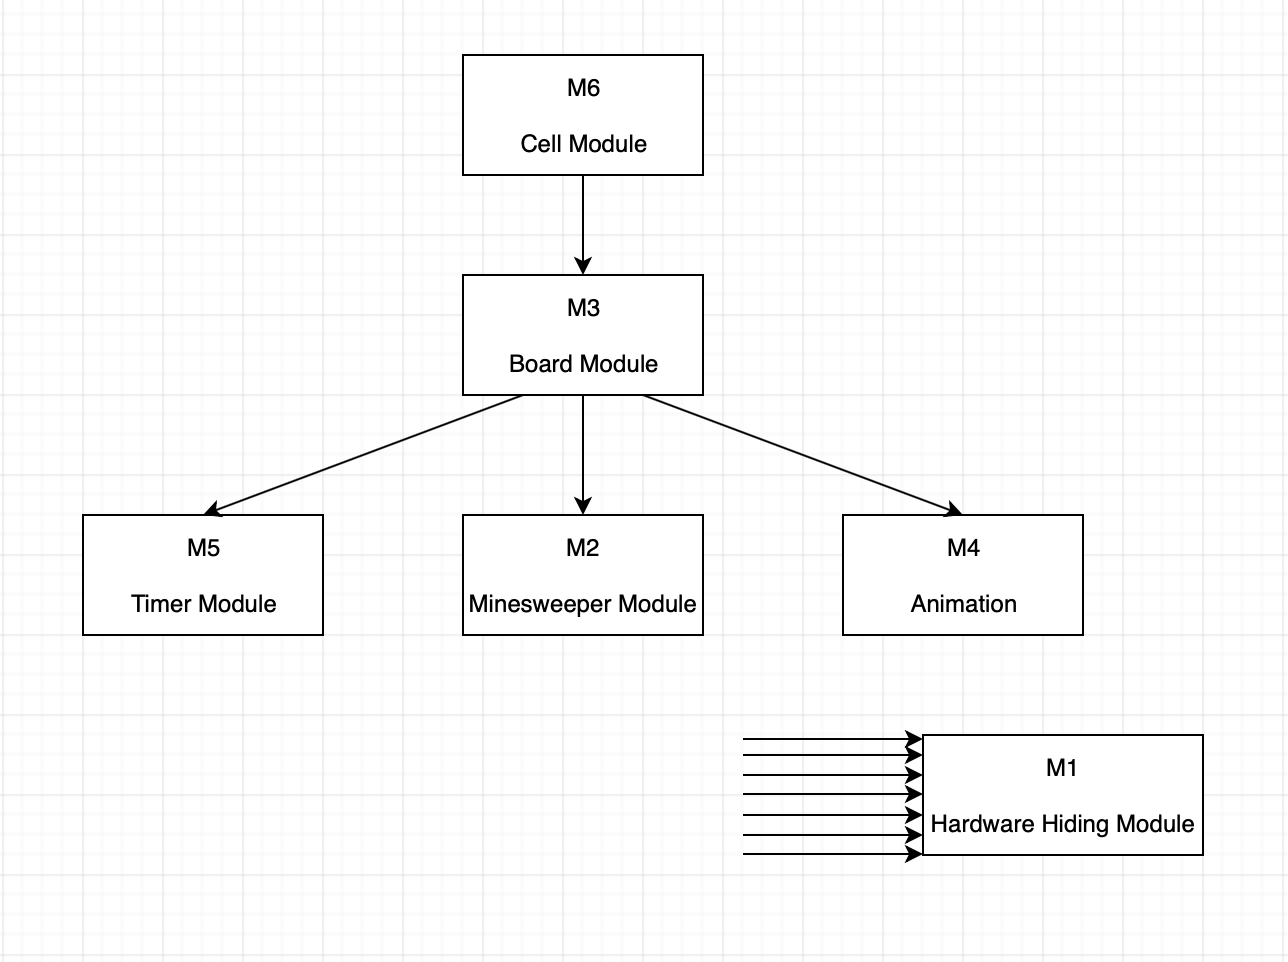
\includegraphics[width=1.0\textwidth]{userh.png}
\caption{Use hierarchy among modules}
\label{FigUH}
\end{figure}

%\section*{References}

\bibliographystyle {plainnat}
\bibliography {MG}

\section{Schedule}
The new Gantt Chart is updated in the Project Schedule folder on git.
\end{document}